\chapter{Parallel optimization}
\label{ch:parallel-optimization}

Optimization algorithms such as SCEM-UA \citep{vrug-gupt-bout-soro-2003}, SODA \citep{vrug-diks-gupt-bout-vers-2005}, Differential Evolution \citep{stor-pric-1997}, or DREAM \citep{vrug-terb-diks-robi-hyma-higd-2009} repeatedly sample the parameter space. In this chapter, we look at how such a sampling algorithm may be parallelized, and we introduce a law that describes the speedup that can be expected from parallelizing\index{parallel} a particular piece of software.

Most parameter optimization algorithms sample the parameter space in generations of independent samples. When the optimization is implemented as a \textit{serial }\index{serial} or \textit{sequential}\index{sequential} algorithm, the members of a generation are evaluated one after the other. For example, if the tasks that need to be evaluated each consist of one parameter set and there are 10 such tasks, the walltime that is needed to evaluate these tasks is equivalent to the sum of the CPU time that individual tasks need (Figure~\ref{fig:walltime-comparison}). In contrast, if the optimization algorithm employs a parallel strategy for evaluating the tasks, and the tasks are started simultaneously on 10 CPUs, then the walltime is determined by the CPU time of the slowest task (including the overhead introduced by the parallelization). The maximum speed-up $S$ that be gained from executing a task in parallel is expressed by \textit{Amdahl's Law}\index{Amdahl's Law}:
\begin{equation}
S=\frac{1}{\alpha}
\label{eq:amdahls-law}
\end{equation}
in which $\alpha$ is the fraction of the program that cannot be parallelized.

For the example in Figure~\ref{fig:walltime-comparison}, each task is about 10\% of the total walltime when executed sequentially, so $\alpha$ is about 0.1 (not counting the overhead due to parallelization), therefore the theoretical maximum speedup is about 10x. When executed in parallel, a relatively large part of the time is spent in communication (`parallelization overhead'). When this is the case, the application is said to be \textit{fine-grained}\index{fine-grained}. In contrast, if a parallel implementation of a program spends most of its time on calculation (as opposed to on communication), it is said to be \textit{coarse-grained}\index{coarse-grained}. Most Monte-Carlo based optimization problems are coarse-grained, since the model CPU time is usually at least a few seconds, or sometimes even hours---in any case, much less than the time needed to send a parameter set over the network. Problems for which the communication time is negligible compared to the calculation time are said to be \textit{embarassingly parallel}\index{embarassingly parallel}.


\begin{figure}[htb]
  \centering
    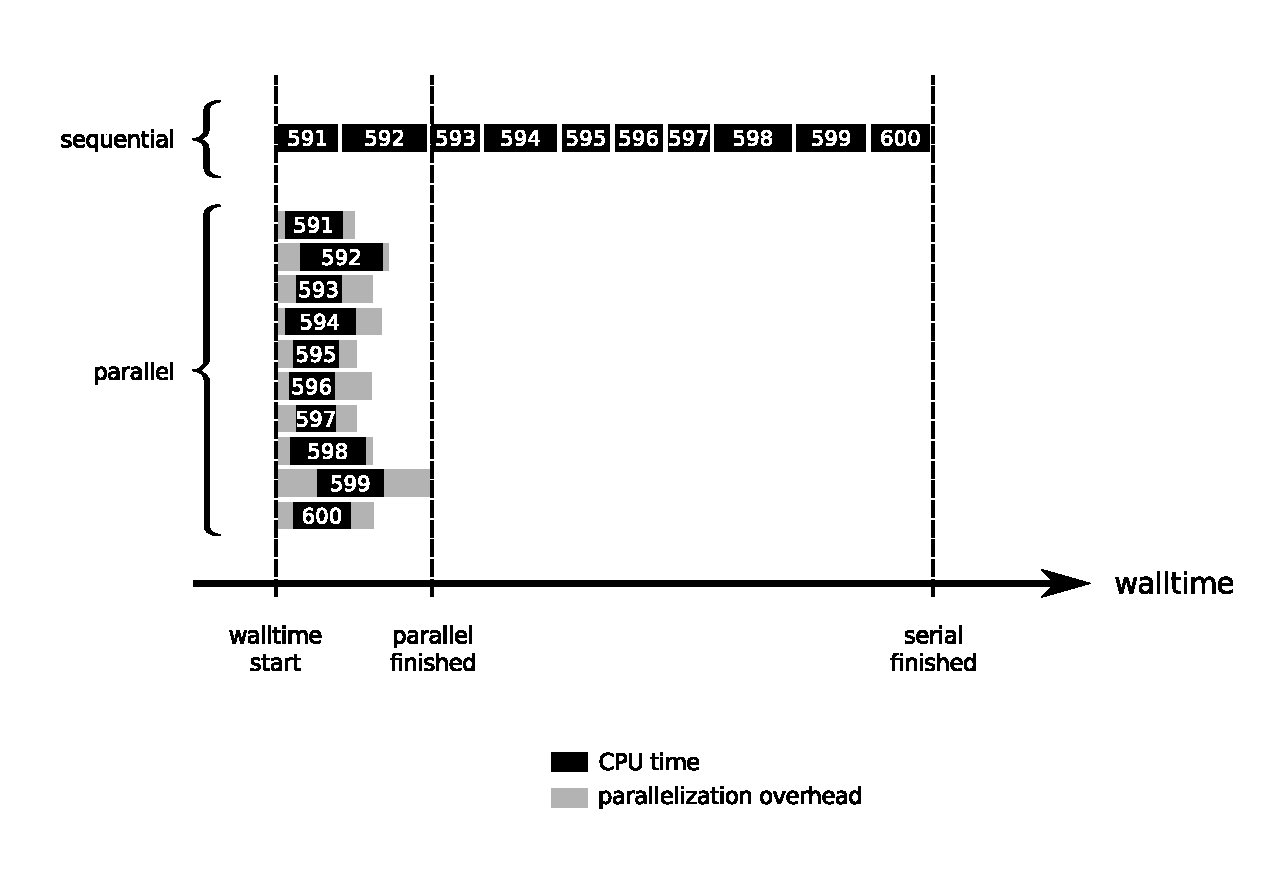
\includegraphics[width=0.9\textwidth]{./../eps/serial-parallel-walltime.eps}
  \caption{Walltime needed to complete 10 tasks 591--600 when evaluated sequentially or in parallel. The actual speedup that is achieved in parallelizing this problem is less than the theoretical maximum speedup due to parallelization overhead. }
  \label{fig:walltime-comparison}
\end{figure}

\section{The Master-Worker paradigm}

For Monte-Carlo type optimization, the Master-Worker paradigm\index{Master-Worker paradigm} (see Fig.~\ref{fig:master-worker-paradigm}; sometimes also referred to as Master-Slave paradigm\index{Master-Slave paradigm}) is the most common. In the Master-Worker paradigm, one of the available nodes is assigned the role of Master, while all the other nodes assume Worker roles.

\subsection{Master side}

The Master node is responsible for keeping track of the status of all Worker nodes with regard to what program a given Worker should run next, as well as to the logistics of the optimization, i.e.\,whether all nodes are connected, which nodes are busy calculating, which have finished, which are waiting for a new task, etc. Furthermore, the Master node is the brains of the optimization algorithm: the Master decides which tasks should be evaluated next. At the very beginning of the optimization, the Master typically checks whether all the nodes are online. After that, the Master will send each node all data that the Worker needs to complete its tasks. This typically includes things like the observations against which the model result will be compared, as well as the model's initial and boundary conditions---basically everything that is constant for all tasks. The Master also sends the model structure itself. Once all Workers have received the data and the model structure, the Master node determines what parameter combinations need to be sampled first. This is entirely dependent on which algorithm is used for the optimization. In any case, the Master compiles a list of all parameter combinations that need to be evaluated (i.e.\,for which the model structure needs to be run). It then distributes these parameter combinations over the available Workers, and waits for the Workers to start returning results. A result is usually in the form of an objective score or likelihood function value, but can in principle be any variable, or even a collection of variables.

\subsection{Worker side}


On the Worker side, things are pretty simple: when the Worker starts, it loads all the initial and boundary conditions that it received from the Master, after which it goes into a never-ending loop. The never-ending loop consists of just a few components: first, it waits for a new task, i.e.\,, a new parameter combination. Once it has received the parameter combination, it runs the model structure with the parameter combination it just received. After the model finishes, the Worker will typically run some sort of objective function to calculate the likelihood function value, for instance by comparing it to observations (which the Master sent to the Worker at the very beginning). The objective function's result is then sent back to the Master node, and the Worker returns to the beginning of the never-ending loop where it either continues with the next task, or waits until it receives a new one.




\begin{figure}[htb]
  \centering
    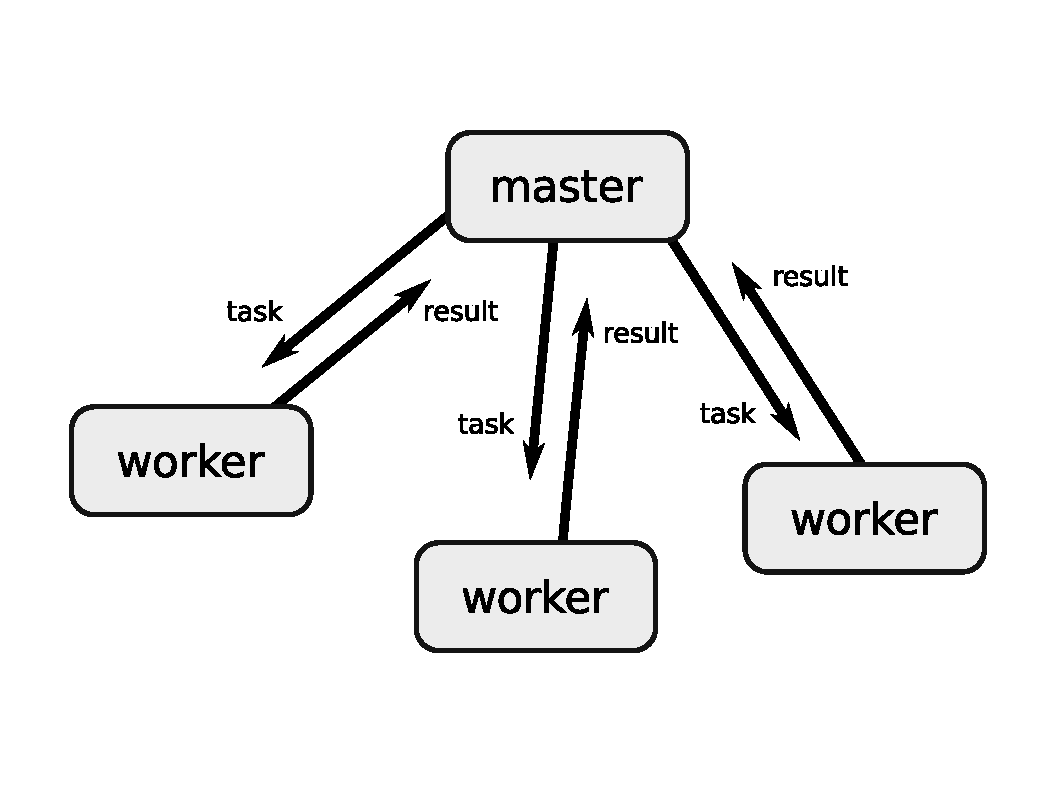
\includegraphics[width=0.9\textwidth]{./../eps/master-worker-paradigm.eps}
  \caption{Message passing between a master node and its workers.}
  \label{fig:master-worker-paradigm}
\end{figure}

